\documentclass[12pt]{article}
\usepackage[utf8]{inputenc}
\usepackage[spanish]{babel}
\usepackage[pdftex]{graphicx}
\usepackage{float}
\usepackage{booktabs}
\usepackage[table,xcdraw]{xcolor}
\usepackage{ltxtable}
\usepackage{proof}
\usepackage{amsmath}
\usepackage{ amssymb }
\usepackage{pdfpages}
\usepackage[left=2cm, right=2cm, top=2cm]{geometry} 
\begin{document}
\begin{titlepage}

\begin{minipage}{2.6cm}

\includegraphics[width=\textwidth]{fceia.pdf}
\end{minipage}
\hfill
%
\begin{minipage}{6cm}
\begin{center}
\normalsize{Universidad Nacional de Rosario\\
Facultad de Ciencias Exactas,\\
Ingeniería y Agrimensura\\}
\end{center}
\end{minipage}
\hspace{0.5cm}
\hfill
\begin{minipage}{2.6cm}

\includegraphics[width=\textwidth]{unr.pdf}
\end{minipage}

\vspace{0.5cm}

\begin{center}
\normalsize{\sc Teoría de Bases de Datos}\\
\vspace{0.5cm}
\large{Trabajo Práctico 1}\\

\Large{\bf Modelado de Datos}\\
\vspace{5cm}

\normalsize
Román Castellarin\\
Gianfranco Paolini\\
Juan Ignacio Suarez\\


\vspace*{0.5cm}
\small{ \today }


\end{center}
\end{titlepage}
\newpage
\section{Diagrama Entidad-Relación}
Para realizar el diagrama Entidad-Relación del problema planteado utilizamos el programa \textsc{Dia}.
\textit{(Ver diagrama adjunto TBD-TP1.dia)}

\begin{figure}[H]
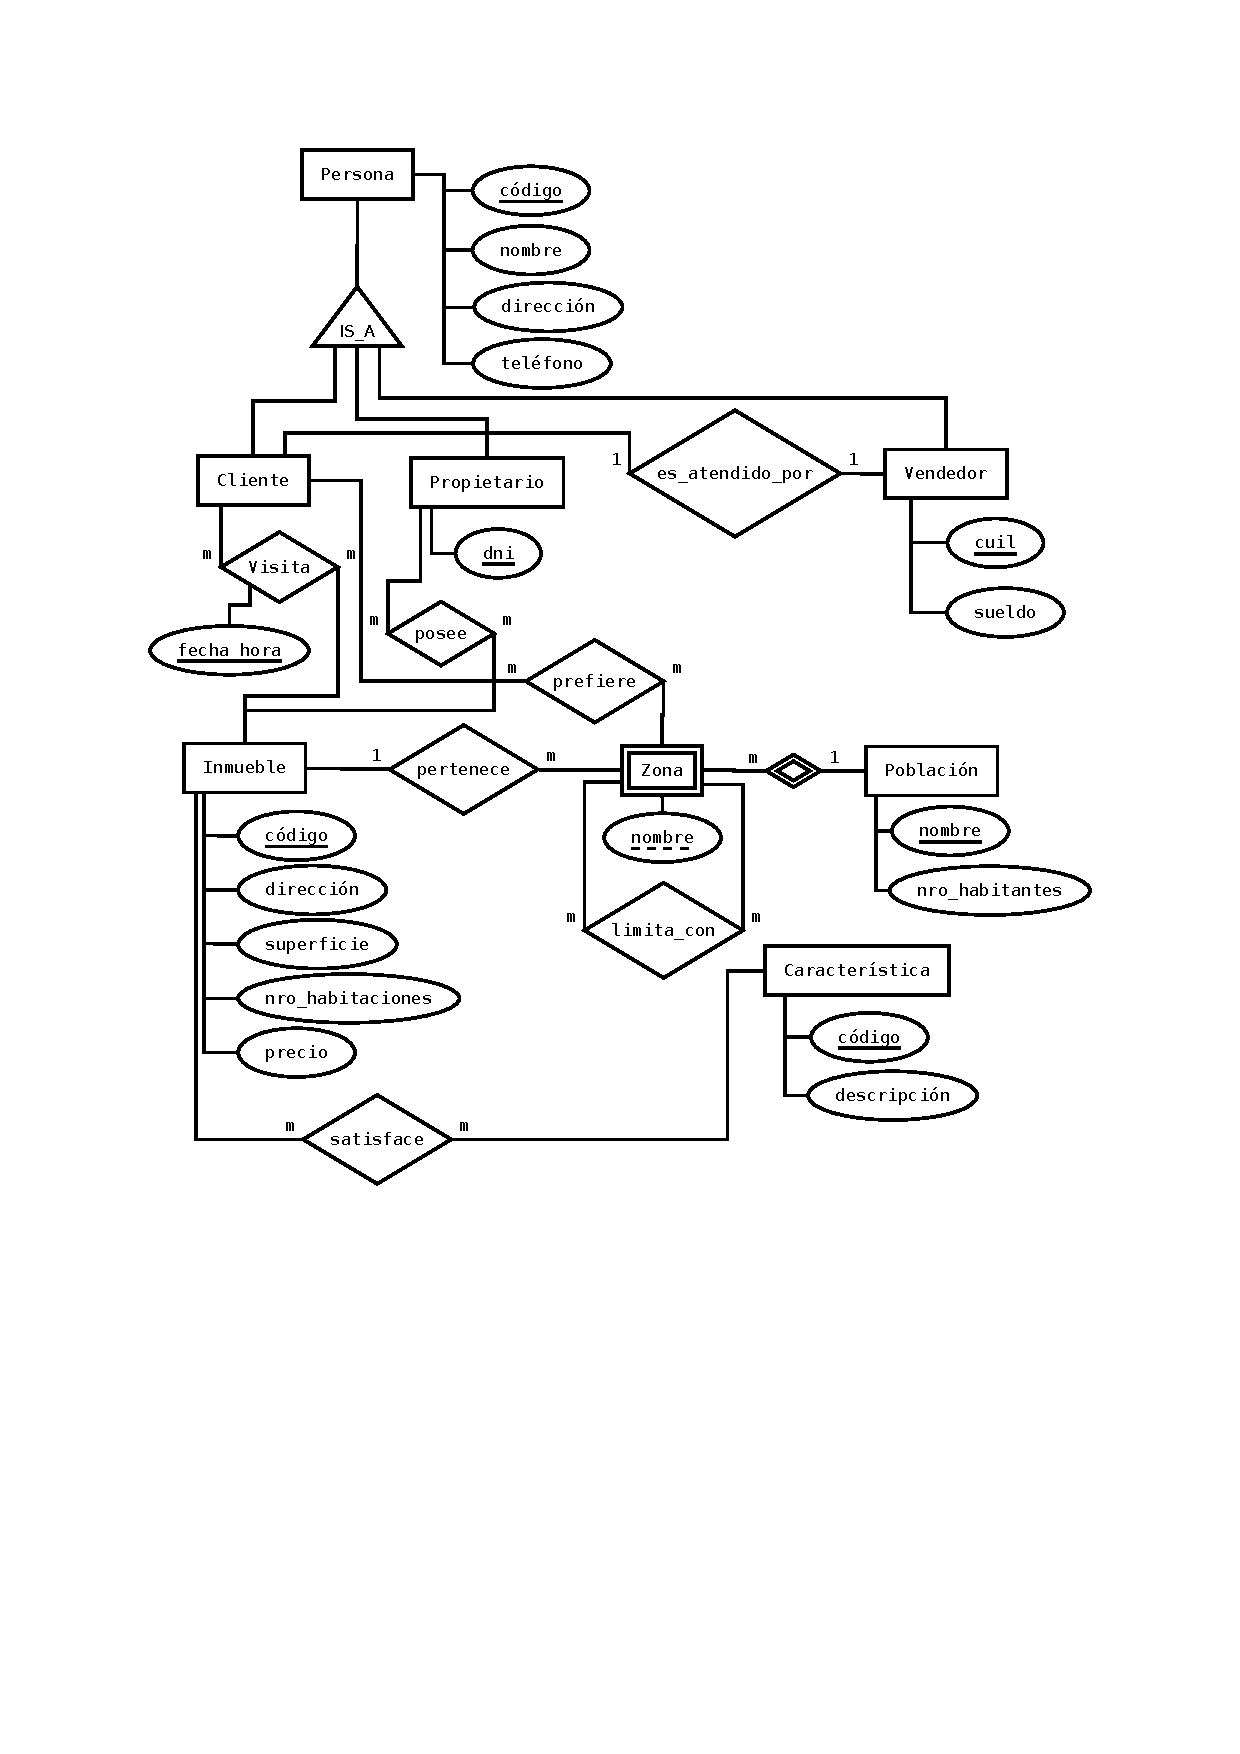
\includepdf[pages=-, offset=0cm -3cm]{ERD.pdf}
%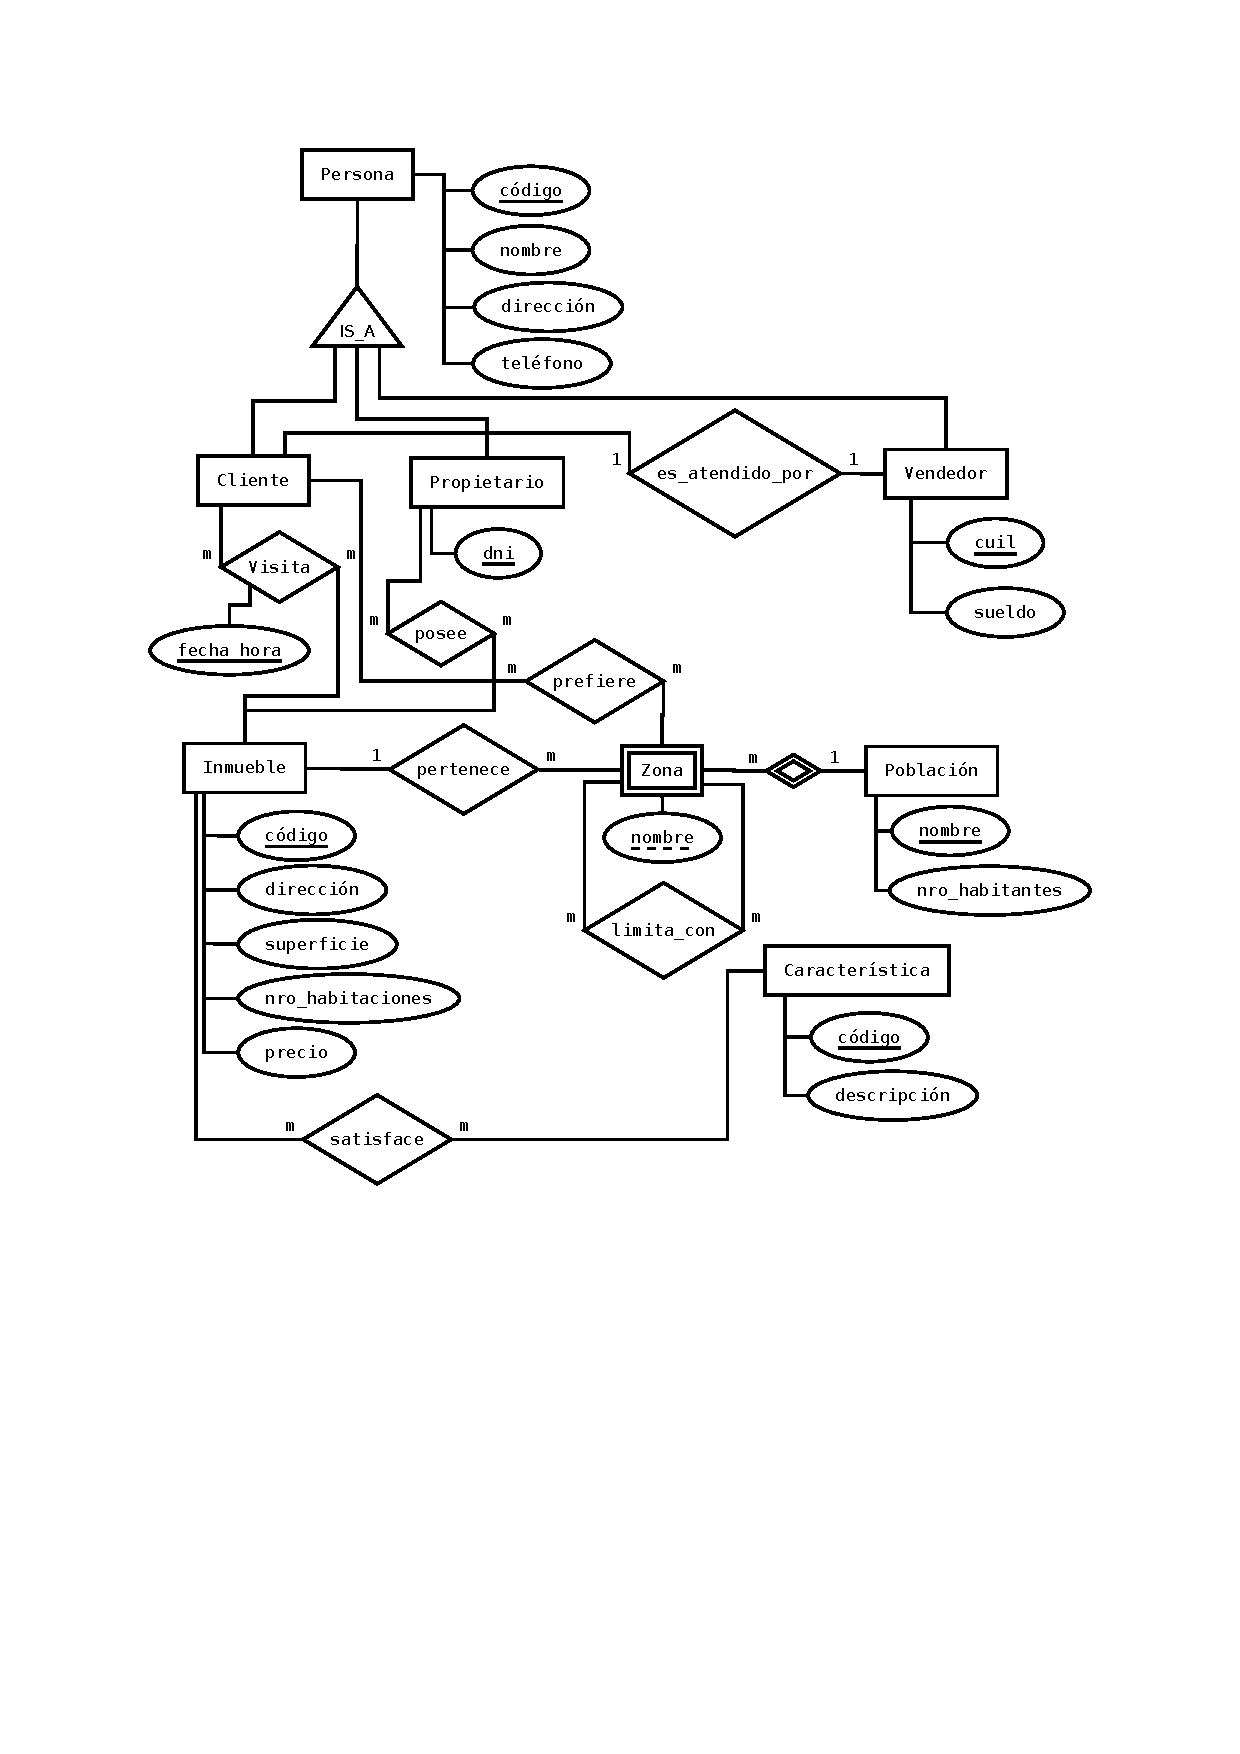
\includegraphics[scale=.8]{ERD.pdf}

\end{figure}
\newpage
\section{Pasaje a tablas en MySQL Workbench}
Para el diseño de las tablas, siguiendo la descripción del trabajo práctico, hemos elegido comprimir la información de \textsc{Propietario}, \textsc{Cliente} y \textsc{Vendedor} en una tabla \textsc{Persona}. Por esto, es responsabilidad del programador mantener las siguientes invariantes:

\begin{itemize}
\item
En la tabla \textsc{Persona} la columna \textsc{Vendedor} tiene que hacer referencia a una fila correspondiente a un \textsc{Vendedor}.
\item
Análogamente sucede con las tablas \textsc{posee} y \textsc{visita}.
\end{itemize}

\textit{(Ver archivo adjunto ER.mwb)}

\vspace{3cm}
\hspace{-5cm}
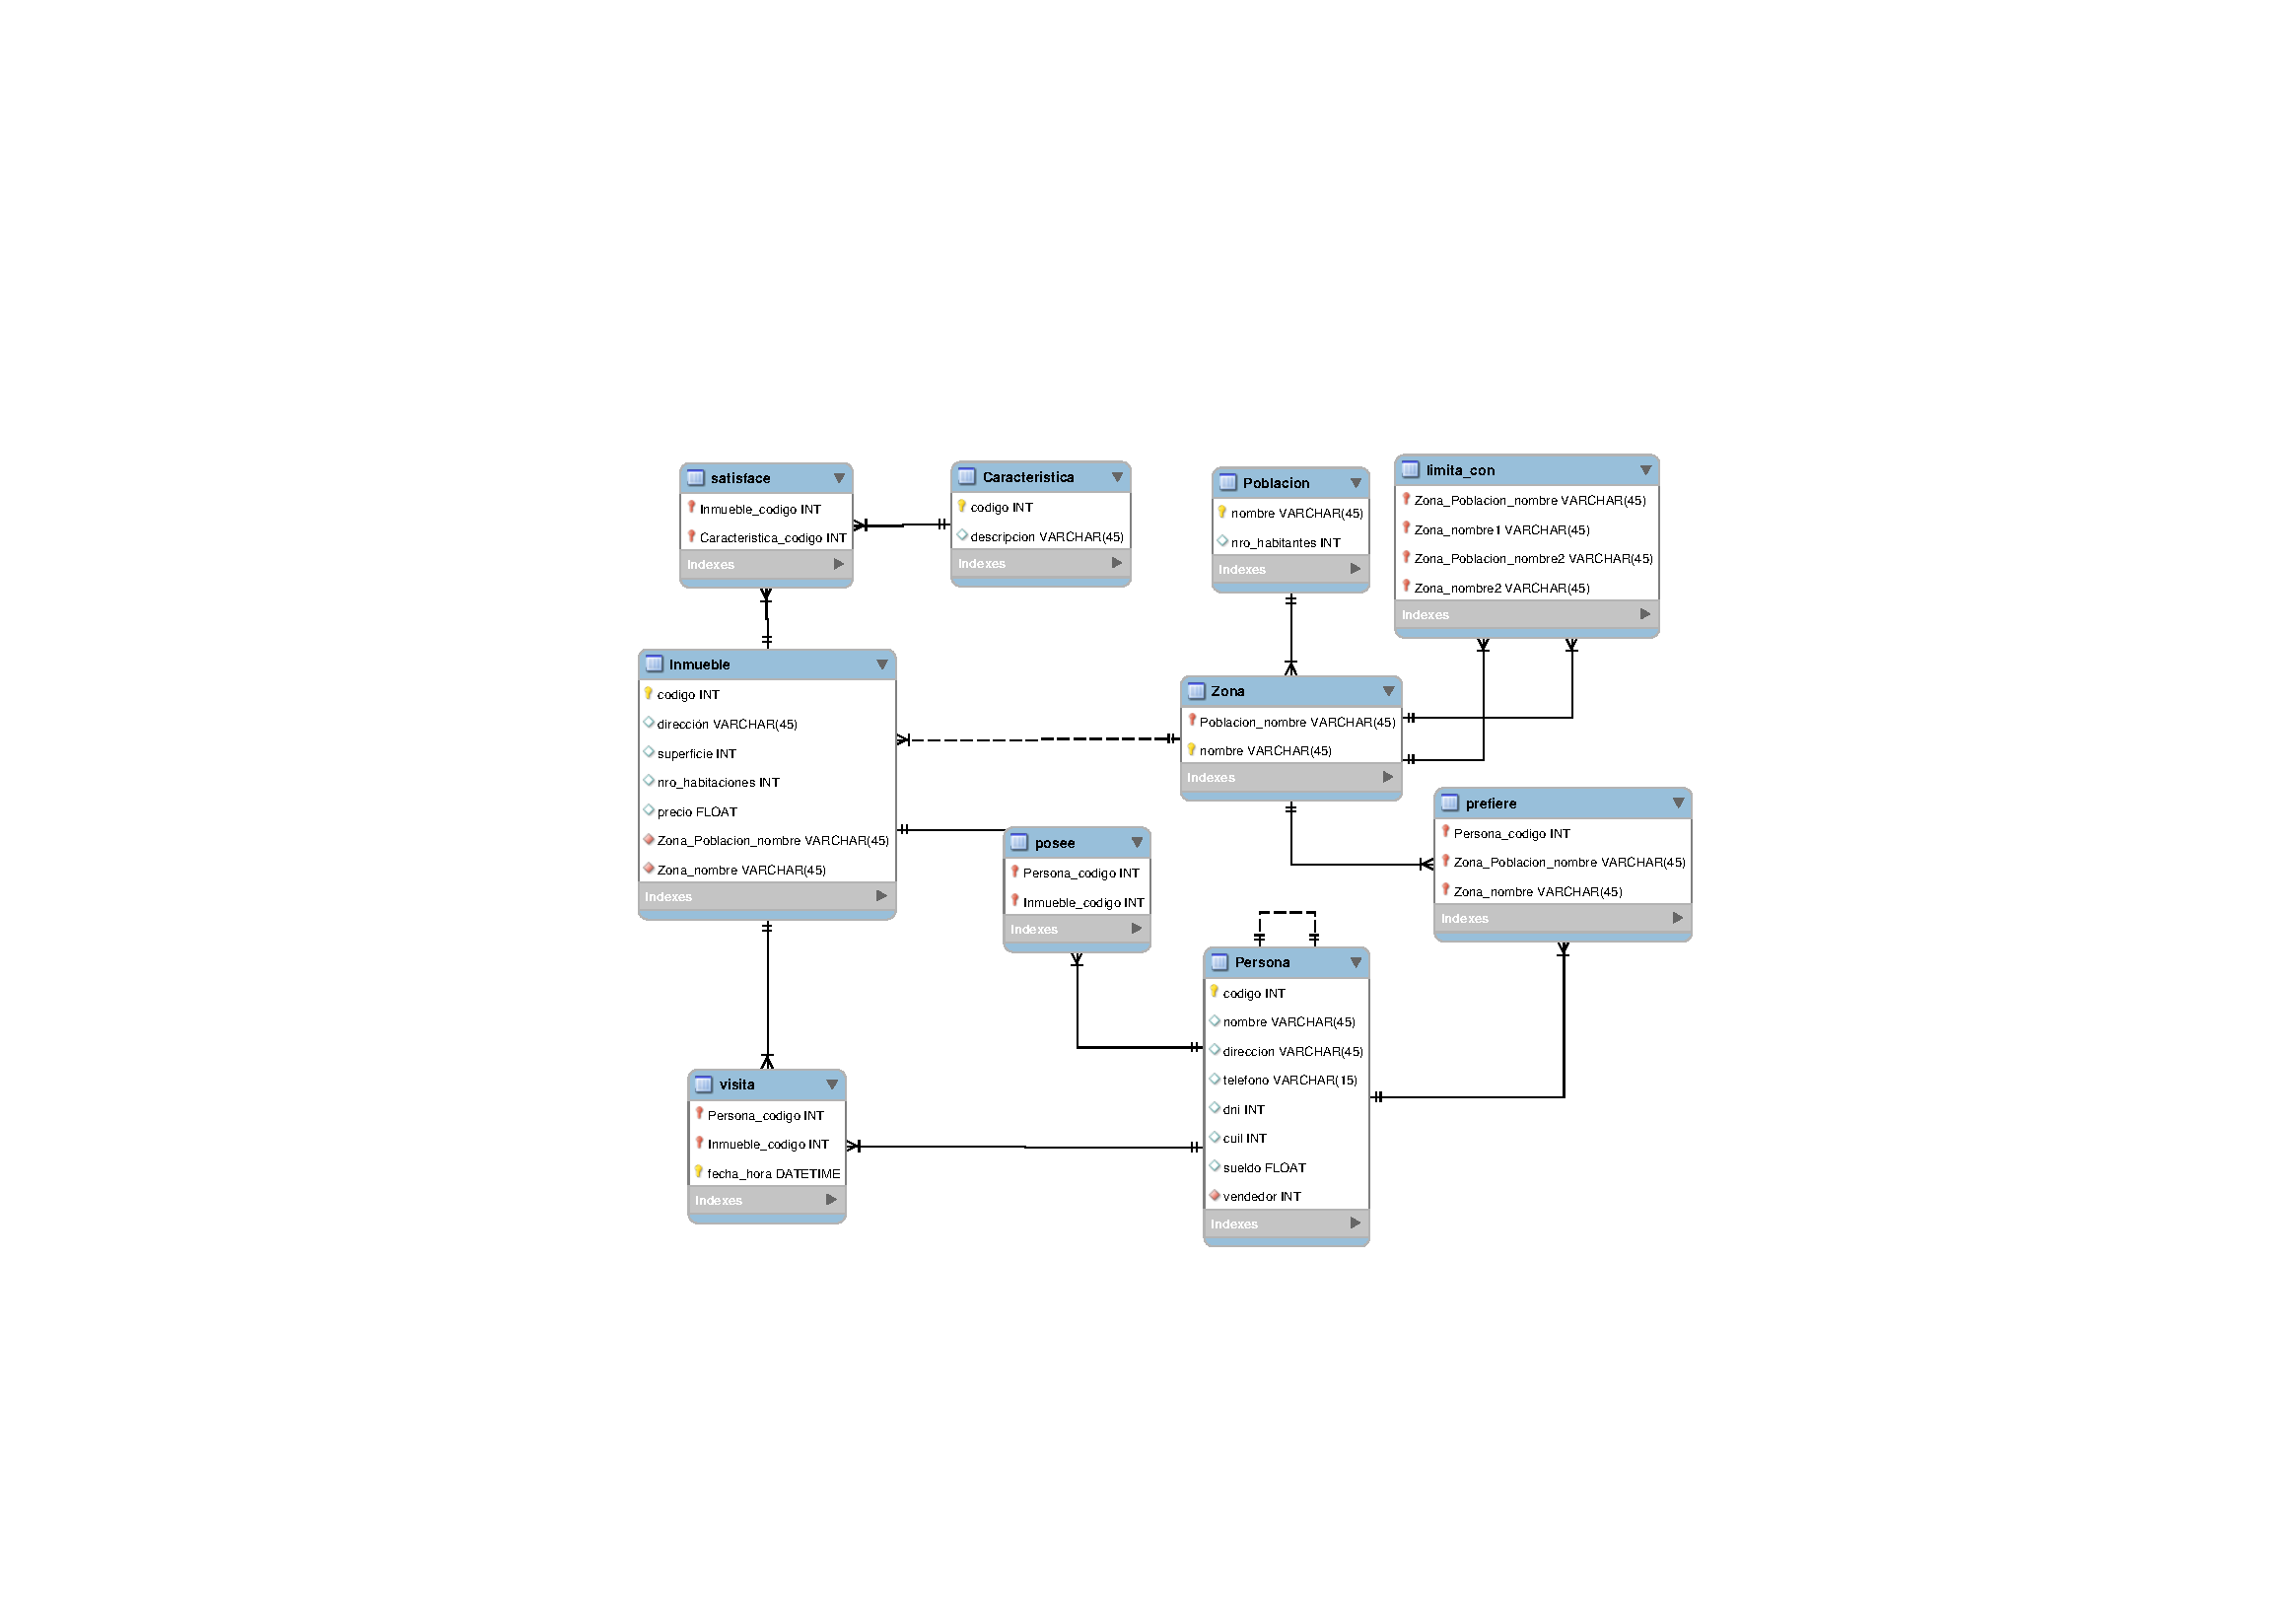
\includegraphics[scale=.7, trim=0.5cm 11cm 0.5cm 11cm]{ER.pdf}

\end{document}
